% Author: Till Tantau
% Source: The PGF/TikZ manual
\documentclass[border=10pt]{standalone}

\usepackage[latin1]{inputenc}
\usepackage{tikz}

% GNUPLOT required
\begin{document}
\pagestyle{empty}
\thispagestyle{empty}

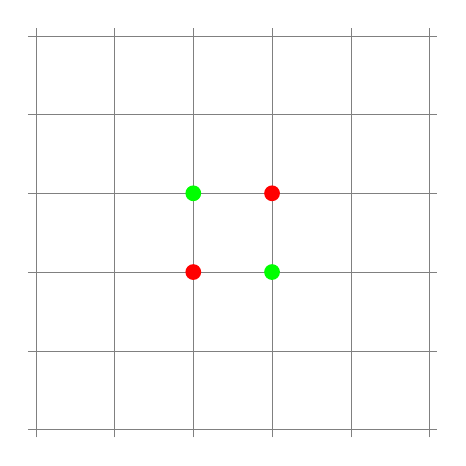
\begin{tikzpicture}[domain=-2:3,smooth, samples=400]
    \draw[very thin,color=gray] (-2.1,-2.1) grid (3.1,3.1);
    %\draw[->] (-0.2,0) -- (4.2,0) node[right] {$x$};
    %\draw[->] (0,-1.2) -- (0,4.2) node[above] {$f(x)$};
    %\draw[color=red] plot[id=x] function{x} 
    %    node[right] {$f(x) =x$};
    %\draw[color=blue] plot[id=asd] function{(1+(1-2*(x-1))/(2+5.5*(x-1)))/2 } node[right] {$f(x) = \sin x$};

    %\draw[color=blue, domain=-2:0.385] plot[id=asd] function{ (1-2*x)/(2-5*x)} node[right]{};
    %\draw[color=blue, domain=0.416:3] plot[id=asd2] function{ (1-2*x)/(2-5*x)} node[right]{};
    \draw[color=blue, domain=-2:3] plot[id=asd] function{x+0.5} node[right]{};

    %\draw[color=orange] plot[id=exp] function{0.05*exp(x)} 
    %    node[right] {$f(x) = \fracf{1}{20} \mathrm e^x$};

    \path [draw=none,fill=green] (1,0) circle (0.1);
    \path [draw=none,fill=green] (0,1) circle (0.1);
    \path [draw=none,fill=red] (0,0) circle (0.1);
    \path [draw=none,fill=red] (1,1) circle (0.1);
\end{tikzpicture}


\end{document}
